
% \begin{enumerate}
% %\begin{multicols}{2}
% \item
% \begin{align}
% \begin{split}
% \myvec{2 & 1 }\vec{x}&=6
% \\
% \myvec{4  & -2}\vec{x}&=4 \label{linform/2/8/2/1.0.1}
% \end{split}
% \end{align}
% \item
% \begin{align}
% \begin{split}
% \myvec{2 & -2 }\vec{x}&=2
% \\
% \myvec{4 & -4 }\vec{x}&=5 \label{linform/2/8/2/1.0.2}
% \end{split}
% \end{align}
% %\end{multicols}
% \end{enumerate}
%
%\begin{enumerate}
\item
\begin{align}
\begin{split}
\myvec{2 & 1 }\vec{x}&=6
\\
\myvec{4 & -2 }\vec{x}&=4
\end{split}
\end{align}
The above equations can be expressed as the matrix equation
\begin{align}
\myvec{2 & 1\\4 & -2} \vec{x} = \myvec{6\\4}
\end{align}
%
The augmented matrix for the above equation is row reduced as follows
\begin{align}
\myvec{2 & 1 & 6\\4 & -2 & 4} 
\xleftrightarrow{R_2\rightarrow \frac{R_1}{2}-\frac{R_2}{4}}
\myvec{2 & 1 & 6\\0 & 1 & 2}
\\
\myvec{2 & 1 & 6\\0 & 1 & 2}
\xleftrightarrow{R_1\rightarrow R_1-R_2}
\myvec{2 & 0 & 4\\ 0 & 1 & 2}
\\
\myvec{2 & 0 & 4\\0 & 1 & 2}
\xleftrightarrow{R_1\rightarrow\frac{R_1}{2}}
\myvec{1 & 0 & 2\\0 & 1 & 2}
\end{align}
%
$\because$ row reduction of the $2\times 3$ matrix
%
\begin{align}
\myvec{2 & 1 & 6\\4 & -2 & 4}
\end{align}
%
results in a matrix with 2 nonzero row, its rank is 2. 
%
Similarly, the rank of the matrix 
\begin{align}
\myvec{2 & 1 \\4 & -2 } 
\end{align}
%
is also 2.
%
\begin{align}
\because Rank \myvec{2 & 1\\4 & -2} &= Rank\myvec{2 & 1 & 6\\4 & -2 & 4}=2\nonumber\\
&=dim\myvec{2 & 1\\4 & -2}=2
\end{align}
$\therefore$ the  lines in \eqref{linform/2/8/2/1.0.1}  intersect as can be seen from Fig.     \ref{linform/2/8/2/fig: INTERSECTING LINES.}

\begin{figure}[ht!]
    \centering
    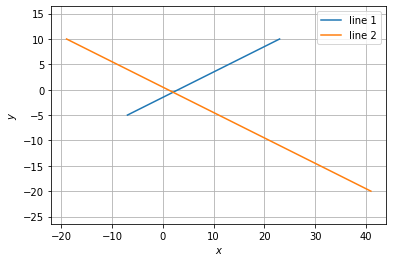
\includegraphics[width=\columnwidth]{solutions/su2021/2/8/2/intersecting lines.png}
    \caption{INTERSECTING LINES}
    \label{linform/2/8/2/fig: INTERSECTING LINES.}
\end{figure} 

\item
\begin{align}
\begin{split}
\myvec{2 & -2 }\vec{x}&=2
\\
\myvec{4 & -4 }\vec{x}&=5
\end{split}
\end{align}
The above equations can be expressed as the matrix equation
\begin{align}
\myvec{2 & -2\\4 & -4} \vec{x} = \myvec{2\\5}
\end{align}
%
The augmented matrix for the above equation is row reduced as follows
\begin{align}
\myvec{2 & -2 & 2\\4 & -4 & 5 } 
\xleftrightarrow{R_2 \rightarrow R_2-2R_1}
\myvec{2 & -2 & 2\\ 0 & 0 & 1}
\end{align}
%
$\because$ row reduction of the $2\times 3$ matrix
%
\begin{align}
\myvec{2 & -2 & 2\\4 & -4 & 5}
\end{align}
%
results in a matrix with 2 nonzero rows, its rank is 2. 
%
Similarly, the rank of the matrix 
\begin{align}
\myvec{2 & -2 \\4 & -4 } 
\end{align}
%
is also 1.
%
\begin{align}
\because Rank \myvec{2 & -2\\4 & -4} \ne Rank\myvec{2 & -2 & 2\\4 & -4 & 5}=1\nonumber\\<dim\myvec{2 & -2\\4 & -4}=2
\end{align}
$\therefore$ the lines in  \eqref{linform/2/8/2/1.0.2}  are parallel as can be seen in Fig.     \ref{linform/2/8/2/fig: PARALLEL LINES.}
%
\begin{figure}[ht]
    \centering
   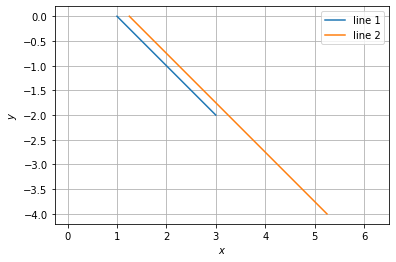
\includegraphics[width=\columnwidth]{solutions/su2021/2/8/2/parallel lines.png}
    \caption{PARALLEL LINES}
    \label{linform/2/8/2/fig: PARALLEL LINES.}
\end{figure}    
\end{enumerate}
